\documentclass[tikz,border=10pt]{standalone}
\usepackage{tikz}
\usetikzlibrary{positioning}
\usepackage{tikz-feynman} % texdoc tikz-feynman 
\usepackage{pgfplots}
\pgfplotsset{width=7cm,compat=1.16}\usepgfplotslibrary{groupplots}
\begin{document}

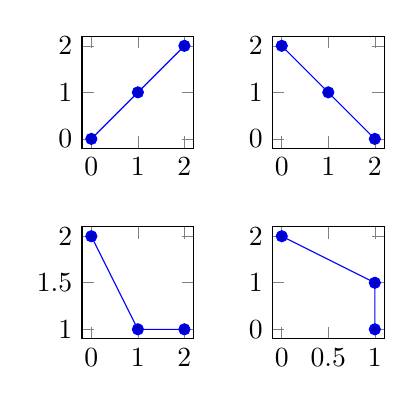
\begin{tikzpicture}
\begin{axis}[name=plot1,height=3cm,width=3cm]
\addplot coordinates {(0,0) (1,1) (2,2)};
\end{axis}
\begin{axis}[name=plot2,at={($(plot1.east)+(1cm,0)$)},anchor=west,height=3cm,width=3cm]
\addplot coordinates {(0,2) (1,1) (2,0)};
\end{axis}
\begin{axis}[name=plot3,at={($(plot1.south)-(0,1cm)$)},anchor=north,height=3cm,width=3cm]
\addplot coordinates {(0,2) (1,1) (2,1)};
\end{axis}
\begin{axis}[name=plot4,at={($(plot2.south)-(0,1cm)$)},anchor=north,height=3cm,width=3cm]
\addplot coordinates {(0,2) (1,1) (1,0)};
\end{axis}
\end{tikzpicture}

\end{document}